\documentclass[border=6pt]{standalone}
\usepackage[T1]{fontenc}
\usepackage{lmodern}
\usepackage{tikz}
\usetikzlibrary{arrows.meta,positioning,shapes.geometric,calc,fit}
\begin{document}
\hyphenpenalty=10000 \exhyphenpenalty=10000
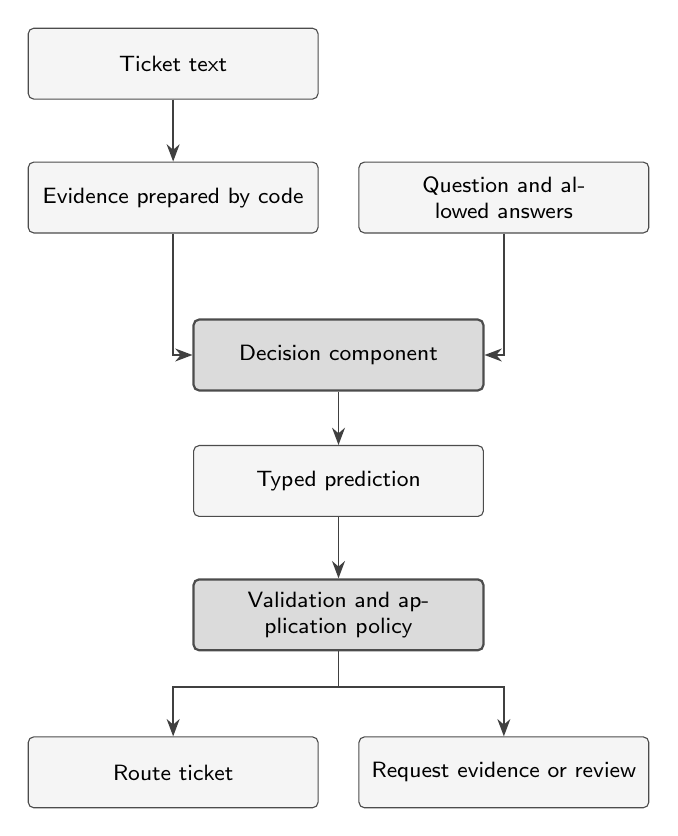
\begin{tikzpicture}[
  font=\footnotesize\sffamily,
  box/.style={draw=black!70, rounded corners=2pt, fill=black!4, align=center,
              text width=3.4cm, minimum height=0.9cm, inner sep=4pt},
  key/.style={box, fill=black!14, line width=0.8pt},
  arr/.style={-{Stealth[length=2.2mm]}, draw=black!75, line width=0.6pt}
]
\node[box] (t) at (-2.1,0) {Ticket text};
\node[box] (e) at (-2.1,-1.7) {Evidence prepared by code};
\node[box] (q) at (2.1,-1.7) {Question and allowed answers};
\node[key] (m) at (0,-3.7) {Decision component};
\node[box] (p) at (0,-5.3) {Typed prediction};
\node[key] (v) at (0,-7.0) {Validation and application policy};
\node[box] (r) at (-2.1,-9.0) {Route ticket};
\node[box] (h) at (2.1,-9.0) {Request evidence or review};

\draw[arr] (t) -- (e);
\draw[arr] (e.south) |- (m.west);
\draw[arr] (q.south) |- (m.east);
\draw[arr] (m) -- (p);
\draw[arr] (p) -- (v);
\draw[arr] (v.south) -- ++(0,-0.45) -| (r.north);
\draw[arr] (v.south) -- ++(0,-0.45) -| (h.north);
\end{tikzpicture}
\end{document}
